\documentclass[11pt,a4paper]{article}
\usepackage[margin=25mm]{geometry}
\usepackage{amsmath,amssymb,amsthm,graphicx,booktabs,xcolor,hyperref}
\definecolor{plum}{HTML}{653856}
\hypersetup{colorlinks=true,urlcolor=plum,linkcolor=plum,citecolor=plum,pdfauthor={Anonymous},pdftitle={The least functional dependence at negative footrule: the lower boundary of the region of Chatterjee's rank correlation and Spearman's footrule}}
\newtheorem{theorem}{Theorem}
\newtheorem{lemma}[theorem]{Lemma}
\newtheorem{corollary}[theorem]{Corollary}
\newtheorem{proposition}[theorem]{Proposition}
\newtheorem{conjecture}[theorem]{Conjecture}
\theoremstyle{remark}
\newtheorem{remark}[theorem]{Remark}
\newcommand{\E}{\mathbb E}
\newcommand{\1}{\mathbf 1}
\newcommand{\R}{\mathbb R}
\newcommand{\dd}{\,\mathrm d}
\DeclareMathOperator{\Law}{Law}
\setlength{\emergencystretch}{2em}
\title{The least functional dependence at negative footrule:\\ the lower boundary of the region of Chatterjee's rank correlation and Spearman's footrule}
\author{Anonymous\\[3pt]{\small DOI \href{https://doi.org/10.5281/zenodo.24538662}{10.5281/zenodo.24538662}}}
\date{24 November 2026}
\begin{document}
\maketitle
\begin{abstract}
The population version of Chatterjee's rank correlation $\xi$ measures how nearly one continuous variable is a function of another, and Spearman's footrule $\psi$ measures how close the two sets of ranks are. Rockel described the set of pairs $(\xi,\psi)$ that can occur together, except for its curved lower edge: for a prescribed negative footrule, the least possible value of $\xi$ was unknown. We determine that edge. For every footrule value strictly between $-1/2$ and $0$ the least value of $\xi$ is attained by exactly one copula, which we construct. Its conditional quantile takes one of two values according to a threshold, and the threshold solves a linear integral equation with a triangular kernel. A dual inequality proves optimality over all copulas, and a quadratic stability estimate shows that nearly optimal copulas are close to the extremiser. The boundary has an elementary closed form when $\psi\le-0.4565\ldots$, a finite piecewise-elementary evaluation elsewhere, and explicit expansions at both ends; for example $\xi+2\psi\ge-0.6042071\ldots$ for every copula. This completes the attainable region. Within it, every pair has a radially symmetric representative. Under positive or negative quadrant dependence we determine the full regions: at zero footrule the attainable values of $\xi$ are $[0,1/2)$ and $[0,3/4)$ respectively, and neither supremum is attained. For stochastically decreasing copulas the lower edge is the same curve, $\psi=0$ forces independence, and every pair with $\xi\le-2\psi$ above the curve is attained; we conjecture that $\xi\le-2\psi$ is the exact upper edge. The construction extends to transport problems with nonuniform margins and to several displacement terms.
\end{abstract}

\section{Introduction}\label{sec:intro}
This section explains the question, what was known, what this paper adds and where each part is proved.

\paragraph{The question.} Let $X$ and $Y$ be continuous random variables and let $U=F_X(X)$ and $V=F_Y(Y)$ be their ranks, scaled to be uniform on $[0,1]$. Two quite different summaries of their dependence are in use. Chatterjee's rank correlation $\xi$ \cite{chatterjee}, whose population version was introduced earlier by Dette, Siburg and Stoimenov \cite{dette}, asks how nearly $Y$ is a function of $X$: it is $0$ exactly under independence and $1$ exactly when $Y$ is almost surely a measurable function of $X$, whether monotone or not. Spearman's footrule $\psi=1-3\E|U-V|$ asks how close the two ranks are on average: it equals $1$ when the ranks agree, $0$ under independence, and its least value is $-1/2$, reached when the ranks always lie in opposite halves. A natural question is how much one summary constrains the other: which pairs $(\xi,\psi)$ can occur together? The answer, the \emph{exact region} of the pair, gives every sharp inequality between the two coefficients. Exact regions have recently been determined for $\xi$ and Spearman's rho \cite{ar}, for $\xi$ and Blomqvist's beta \cite{olr}, and for several classical pairs of concordance measures (see the references in \cite{rockel,ar2}).

\paragraph{What was known.} Rockel \cite{rockel} studied the pair $(\xi,\psi)$. He proved that the largest footrule compatible with a given $\xi$ is $\sqrt\xi$, attained only by mixtures of independence and comonotonicity; he determined the region for stochastically increasing copulas; and he showed that at the extreme footrule $\psi=-1/2$ the least possible $\xi$ is $1/2$, attained only by a $2\times2$ checkerboard copula. He also proved that the region is convex and closed and that each point of its lower edge is attained by a stochastically decreasing copula \cite[Theorem~3.2]{rockel}, and, in the published version, that $|\psi|\le\sqrt\xi$ for every copula \cite[Corollary~2]{rockel}. The remaining edge, the least $\xi$ for a given footrule in $(-1/2,0)$, was left open: equivalently, the minimum of $\xi+\mu\psi$ over all copulas for $\mu>0$ \cite[eq.~(16)]{rockel}. Rockel bounded it from below by a Jensen relaxation whose minimiser is not a copula, and from above by a two-parameter family of copulas found from discretised optimisation.

\paragraph{What is new.} We determine the open edge exactly (Theorem~\ref{main}). For each multiplier $\mu=2k>0$ the minimum of $\xi+2k\psi$ is attained by one and only one copula $C_k$. In words: draw independent uniforms $U$ and $T$; the response is the lower of two levels $A_k(T)<A_k(T+k)$ when $U$ exceeds a threshold $r_k(T)$, and the upper level otherwise. The threshold is the solution of a linear integral equation with a triangular kernel, and the levels are obtained from it by integration. As $k$ runs from $0$ to $\infty$ these copulas trace the whole curved edge, from independence to the checkerboard. The answer is explicit in the following sense. For $k\ge1$, equivalently $\psi\le-0.4565437\ldots$, it is a closed form in hyperbolic functions (Proposition~\ref{finite}); for $0<k<1$ it is a finite piecewise-elementary calculation; and both ends have explicit expansions, $\psi=-\sqrt\xi+\xi/4+O(\xi^{3/2})$ near independence. Table~\ref{tab:values} lists values and compares them with the two previous lower bounds. Figure~\ref{fig:curve} shows the completed region.

Rockel's feasible family was already close to optimal: for the objective $\xi+\psi$ (that is, $\mu=1$) its best member gives $-0.193$ to the three decimals reported \cite[Table~2]{rockel}, and the exact minimum is $-0.1932281\ldots$. What the present paper supplies is therefore the exact value at every multiplier, a proof of optimality valid for all copulas (including singular ones), the unique extremiser, and a stability estimate saying that copulas with nearly optimal $\xi+2k\psi$ have conditional distribution functions close to those of $C_k$.

The same method settles several restricted versions of the problem (Section~\ref{sec:classes}). Every attainable pair is attained by a radially symmetric copula, as Orenday Lares and Rockel found for the pair $(\xi,\beta)$ \cite{olr}. Under positive quadrant dependence the region is the part of the full region with $\psi>0$ together with the segment $\{(\xi,0):0\le\xi<1/2\}$; under negative quadrant dependence it is the part with $\psi<0$ together with $\{(\xi,0):0\le\xi<3/4\}$. The two zero-footrule sections differ, and neither endpoint is attained. For stochastically decreasing copulas, whose region Rockel noted would need exactly the lower edge found here \cite[Remark~2(e)]{rockel}, we prove that the lower edge is the same curve, that $\psi\le0$ with equality only under independence, and that every pair between the curve and the line $\xi=-2\psi$ is attained. We conjecture that this line is the upper edge, and give numerical evidence. Finally, the transport argument behind the main theorem applies to nonuniform margins and to objectives with several absolute-displacement terms (Section~\ref{sec:transport}).

\paragraph{Method.} The coefficient $\xi$ is quadratic in the conditional distribution functions, which makes direct optimisation awkward. Written through conditional quantiles, however, the objective becomes linear: minimising $\xi+2k\psi$ is the same as maximising $\E\{TV+k(V-U)_+\}$ over couplings of a source $(U,T)$ in the unit square with a uniform target $V$ (Section~\ref{sec:dual}). This is a transport problem from two dimensions to one with a payoff that has a kink at $V=U$. Its two affine branches give a supporting-line (dual) certificate, and the requirement that the target be uniform becomes the linear integral equation (Section~\ref{sec:equation}). The relevant transport theory from several dimensions to one is that of Chiappori, McCann and Pass \cite{cmp}, which assumes smoothness this payoff lacks; duality for costs depending on whole conditional laws goes back to Gozlan, Roberto, Samson and Tetali \cite{gozlan}. Ansari and Rockel used an optimal-transport dual construction for Spearman's rho and footrule \cite{ar2}. Neither the triangular kernel nor the supporting-line inequality is new as a mathematical object; what is new is their combination into an exact solution of this problem.

\paragraph{Roadmap.} Section~\ref{sec:main} fixes notation and states the main theorem. Section~\ref{sec:dual} proves the dual inequality, Section~\ref{sec:equation} solves the threshold equation and proves optimality, uniqueness and stability, and Section~\ref{sec:trace} shows that the extremisers trace the whole edge and completes the region. Section~\ref{sec:eval} gives the closed form, the finite evaluation and the endpoint expansions. Section~\ref{sec:classes} treats radial symmetry, quadrant dependence and stochastic decrease. Section~\ref{sec:transport} gives the transport extensions. Section~\ref{sec:numerics} describes independent numerical checks, and Section~\ref{sec:limits} lists limits and open problems.

\begin{figure}[htbp]
\centering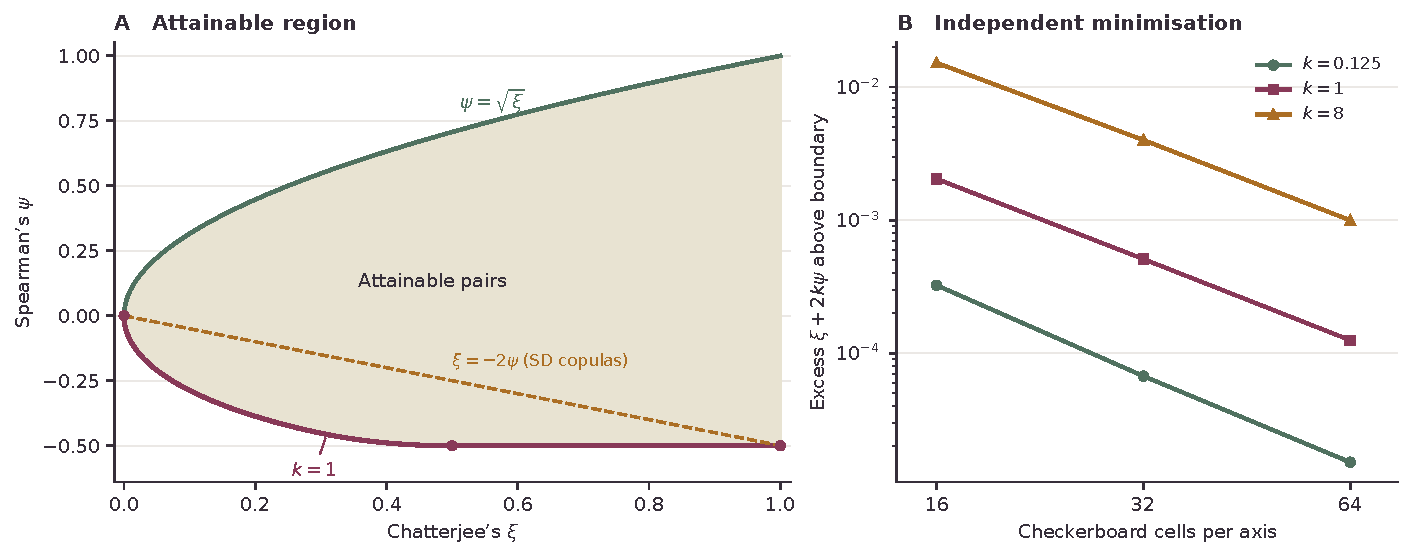
\includegraphics[width=\linewidth]{figures/boundary-figure.pdf}
\caption{Panel A: the attainable region of $(\xi,\psi)$ over all copulas. The upper edge $\psi=\sqrt\xi$ is Rockel's; the curved lower edge from independence $(0,0)$ to the checkerboard $(1/2,-1/2)$ is Theorem~\ref{main}; the dashed line $\xi=-2\psi$ is attained by stochastically decreasing copulas (Proposition~\ref{sdregion}). Panel B: the amount by which the best checkerboard copula on an $n\times n$ grid exceeds the exact minimum of $\xi+2k\psi$ (dimensionless), for three multipliers. The excess falls roughly fourfold per doubling of $n$, consistent with the exact continuum value.}
\label{fig:curve}
\end{figure}

\section{Setting and main result}\label{sec:main}
This section fixes notation, defines the extremal copulas and states the main theorem.

A copula $C$ is the joint distribution function of a pair $(U,V)$ with uniform marginals on $[0,1]$. For $u,v\in[0,1]$ write $h_C(u,v)=\Pr(V\le v\mid U=u)$ for a version of the conditional distribution function; we always use a version that is jointly measurable and right-continuous and nondecreasing in $v$. The population coefficients are
\[
 \xi(C)=6\int_0^1\!\int_0^1 (h_C(u,v)-v)^2\dd u\dd v,
 \qquad \psi(C)=1-3\E|U-V|=6\int_0^1C(t,t)\dd t-2 .
\]
The first expression equals Rockel's $6\iint(\partial_1C)^2-2$, because $\int_0^1h_C(u,v)\dd u=v$. Note that $\xi$ is directional, from $U$ to $V$. Spearman's rho is $\rho(C)=12\E[UV]-3$. We write $\Pi(u,v)=uv$ for independence, $M(u,v)=\min(u,v)$ and $W(u,v)=(u+v-1)_+$. The \emph{attainable region} is $\{(\xi(C),\psi(C)): C \text{ a copula}\}$.

Write $L(s)=\min(1,\max(0,s))$ for the clipping map. For $k>0$ and $t\in[0,1]$ define the averaged clipping function, the triangular integral operator on functions on $[0,1]$, the threshold and the level function:
\begin{align}
 b_k(t)&=\frac1k\int_t^{t+k}L(s)\dd s, &
 (K_kr)(t)&=\int_0^1\Big(1-\frac{|z-t|}{k}\Big)_+r(z)\dd z, \label{kernel}\\
 r_k&=(I+K_k)^{-1}b_k, &
 A_k(s)&=L(s)-\int_{L(s-k)}^{L(s)}r_k(z)\dd z\quad(0\le s\le1+k).\label{solution}
\end{align}
Section~\ref{sec:equation} shows that $I+K_k$ is invertible, with inverse the uniformly convergent series $\sum_{j\ge0}(-K_k)^j$, that $r_k$ is continuous and nondecreasing with values in $[0,1]$, and that $A_k$ is a continuous distribution function on $[0,1+k]$. Let $U,T$ be independent uniforms and put
\[
 V_k=A_k\big(T+k\1_{\{U<r_k(T)\}}\big),\qquad C_k=\Law(U,V_k).
\]
Thus, given $T=t$, the response is the upper level $A_k(t+k)$ if $U<r_k(t)$ and the lower level $A_k(t)$ otherwise. Abbreviating $r=r_k(t)$, $a=A_k(t)$ and $b=A_k(t+k)$, define
\begin{align}
 x_k&=1-6\int_0^1(2t-1)\{(1-r)a+rb\}\dd t,\label{xformula}\\
 y_k&=1-3\int_0^1\{\tfrac12+rb-(1-r)a-r^2\}\dd t.\label{yformula}
\end{align}

\begin{theorem}\label{main}
For each $k>0$, $C_k$ is a copula, it is the unique minimiser of $\xi+2k\psi$ over all copulas, and $(\xi(C_k),\psi(C_k))=(x_k,y_k)$. As $k$ increases from $0$ to $\infty$, $y_k$ decreases continuously and strictly from $0$ to $-1/2$, and $x_k$ increases continuously and strictly from $0$ to $1/2$. Every copula satisfies, and every pair in the following set is attained by some copula:
\[
 -\tfrac12\le y\le1,\qquad m(y)\le x\le1,\qquad
 m(y)=\begin{cases}
 1/2 & y=-1/2,\\
 x_k\ \text{ where } y_k=y & -1/2<y<0,\\
 y^2 & 0\le y\le1.
 \end{cases}
\]
For $-1/2<y<0$ the least value $m(y)$ is attained only by $C_k$; this copula is stochastically decreasing, meaning that its conditional quantiles decrease weakly in $u$. Every copula $C$ satisfies the stability estimate
\begin{equation}
 \xi(C)+2k\psi(C)-x_k-2ky_k
 \ \ge\ 6\|h_C-h_{C_k}\|_{L^2([0,1]^2)}^2. \label{stability}
\end{equation}
\end{theorem}
The upper edge $\psi=\sqrt\xi$ (equivalently $x\ge y^2$ for $y\ge0$), the point $(1/2,-1/2)$ and the segment $\{(x,-1/2):x\ge1/2\}$ are Rockel's \cite{rockel}. The new part is the open arc $0<x<1/2$, $-1/2<y<0$. For example, taking $k=1$ gives the sharp universal inequality $\xi+2\psi\ge x_1+2y_1=-0.6042071213\ldots$; at $\psi=y_1=-0.4565437066\ldots$ the least possible $\xi$ is $x_1=0.3088802920\ldots$. Table~\ref{tab:values} gives the least $\xi$ at selected footrule values.

\begin{table}[htbp]
\centering
\caption{The least attainable $\xi$ at selected negative footrule values (Theorem~\ref{main}), with the parameter $k$ of the extremiser, compared with Rockel's Jensen lower bound \cite[Theorem~3.1]{rockel} and the Cauchy--Schwarz bound $\psi^2$ \cite[Corollary~2]{rockel}. Values are rounded to six decimals; the closed form, the finite-mode evaluation and an independent midpoint solver agree to better than $10^{-6}$ (Section~\ref{sec:numerics}).}
\label{tab:values}
\begin{tabular}{rrrrr}
\toprule
$\psi$ & $k$ & least $\xi$ (exact) & Jensen bound & $\psi^2$\\
\midrule
$-0.05$ & 0.052023 & 0.002566 & 0.002506 & 0.002500\\
$-0.10$ & 0.108761 & 0.010562 & 0.010089 & 0.010000\\
$-0.20$ & 0.241748 & 0.045103 & 0.041338 & 0.040000\\
$-0.30$ & 0.416398 & 0.109988 & 0.096731 & 0.090000\\
$-0.40$ & 0.680931 & 0.217375 & 0.182509 & 0.160000\\
$-0.45$ & 0.931338 & 0.296278 & 0.241056 & 0.202500\\
$-0.49$ & 2.300315 & 0.403996 & 0.299900 & 0.240100\\
\bottomrule
\end{tabular}
\end{table}

\section{A dual inequality from conditional quantiles}\label{sec:dual}
This section rewrites the objective through conditional quantiles, which makes it linear, and proves the supporting-line inequality that certifies optimality.

\paragraph{Conditional quantile representation.} For a copula $C$ let $Q(u,\cdot)$ be the right-continuous generalised inverse of $h_C(u,\cdot)$. A jointly measurable version exists, since each set $\{Q(u,t)\le q\}=\{h_C(u,q)\ge t\}$ with $q$ rational is measurable. If $T$ is uniform and independent of $U$, then $V=Q(U,T)$ has conditional law $h_C(U,\cdot)$, so $(U,V)\sim C$. Let $T'$ be a further independent uniform and $V'=Q(U,T')$, a second draw that is conditionally independent of $V$ given $U$. Integrating over thresholds gives $\E(|V-V'|\mid U=u)=2\int_0^1 h_C(u,v)(1-h_C(u,v))\dd v$, and with $\int_0^1\!\int_0^1 h_C^2=(\xi+2)/6$ this yields
\[
 \xi(C)=1-3\E|V-V'|.
\]
For a nondecreasing function $q$ and independent uniforms $T,T'$, splitting into $T>T'$ and $T<T'$ gives $\E|q(T)-q(T')|=2\int_0^1(2t-1)q(t)\dd t$. Since $Q(u,\cdot)$ is nondecreasing,
\begin{equation}
 \xi(C)=1-6\E[(2T-1)V]=6\E(V-T)^2,\label{xiquantile}
\end{equation}
the last form using $\E V=\E T=1/2$ and $\E V^2=\E T^2=1/3$. Finally $|U-V|=2(V-U)_++U-V$ and $\E U=\E V$, so
\begin{equation}
 \xi(C)+2k\psi(C)=4+2k-12\,\E\{TV+k(V-U)_+\}. \label{objective}
\end{equation}

\paragraph{The relaxed problem.} Consider the larger problem of maximising $\E\{TV+k(V-U)_+\}$ over all joint laws of $(U,T,V)$ in which $(U,T)$ is uniform on the square and $V$ is uniform on $[0,1]$, with no further restriction. Every copula provides such a law, $V=Q(U,T)$, and for it the objective equals $(4+2k-\xi-2k\psi)/12$ by \eqref{objective}. Hence the relaxed maximum is at least the maximum over copulas. Conversely, if a relaxed maximiser has the form $V=q(U,T)$ with $q(u,\cdot)$ nondecreasing for almost every $u$, then $q(u,\cdot)$ is a version of the conditional quantile of $V$ given $U=u$; the law of $(U,V)$ is then a copula $C$, identity \eqref{xiquantile} applies to it, and $C$ minimises $\xi+2k\psi$ over all copulas. Identity \eqref{xiquantile} is used only on the copula side: for a general relaxed law the objective is not $\xi$.

\begin{lemma}\label{dual}
Let $A$ be a continuous nondecreasing function on $[0,1+k]$ with values in $[0,1]$. Set $H(s)=\int_0^s A(z)\dd z$ and $r(t)=(H(t+k)-H(t))/k$. If $A(T+k\1_{\{U<r(T)\}})$ is uniform, it maximises the relaxed problem and is a conditional quantile given $U$.
\end{lemma}
\begin{proof}
Define the convex conjugate $H^*(v)=\sup_{0\le s\le1+k}(sv-H(s))$. The supporting-line inequality gives $sv-H^*(v)\le H(s)$ for all $s,v$, with equality when $v=A(s)$, because $A=H'$. The payoff is the larger of two affine functions of $v$: $tv+k(v-u)_+=\max\{tv,\,(t+k)v-ku\}$. Applying the supporting-line inequality to each branch,
\[
 tv+k(v-u)_+-H^*(v)
 \le \max\{H(t),H(t+k)-ku\}
\]
for all $t,u,v$. Take expectations over any relaxed law. The right side depends only on $(U,T)$, and $\E H^*(V)$ depends only on the uniform law of $V$, so the bound $\E\max\{H(T),H(T+k)-kU\}+\E H^*(V)$ is the same for every relaxed law. The second branch on the right is the larger precisely when $u<r(t)$; the set $\{U=r(T)\}$ is null because $U$ is uniform and independent of $T$. Choosing $v=A(t+k)$ when $u<r(t)$ and $v=A(t)$ otherwise makes both inequalities equalities. Hence the stated $V$ attains the bound, so it maximises the relaxed problem when it is uniform.

Finally, $r$ is a moving average of the nondecreasing function $A$, hence nondecreasing and continuous. For fixed $u$, the map $t\mapsto A(t+k\1_{\{u<r(t)\}})$ can switch only once, from the lower level $A(t)$ up to the upper level $A(t+k)$, as $t$ increases; it is therefore nondecreasing in $t$. Its right-continuous modification is the conditional quantile of $V$ given $U=u$, and the modification changes $V$ only on a null set.
\end{proof}

\section{The threshold equation and its solution}\label{sec:equation}
This section shows that the uniformity condition of Lemma~\ref{dual} is the linear equation $r=b_k-K_kr$, solves it, and derives optimality, uniqueness, the formulae for $(x_k,y_k)$ and the stability estimate.

For any continuous $r:[0,1]\to[0,1]$, the random slope $S=T+k\1_{\{U<r(T)\}}$ takes the value $T+k$ with conditional probability $r(T)$ and $T$ otherwise. Its distribution function is
\[
 A_r(s)=\int_0^1[(1-r(z))\1_{\{z\le s\}}+r(z)\1_{\{z+k\le s\}}]\dd z
       =L(s)-\int_{L(s-k)}^{L(s)}r(z)\dd z,
\]
which is continuous because $S$ has a density. Hence $A_r(S)$ is uniform by the probability integral transform, even if the law of $S$ has a gap. Lemma~\ref{dual} applies with $A=A_r$ provided $r$ is the moving average of $A_r$. By Fubini's theorem,
\[
 \frac1k\int_t^{t+k} A_r(s)\dd s=b_k(t)-K_kr(t),
\]
because a given $z$ is subtracted for $s\in[z,z+k]\cap[t,t+k]$, an interval of length $(k-|z-t|)_+$. So the condition is the linear equation $r+K_kr=b_k$.

\paragraph{Existence and computation.} The map $r\mapsto b_k-K_kr$ sends the closed set of continuous $[0,1]$-valued functions into itself, because its value at $t$ is the average of the distribution function $A_r$ over $[t,t+k]$. Its Lipschitz constant in the supremum norm is at most
\[
 q_k=\sup_t\int_0^1\Big(1-\frac{|z-t|}{k}\Big)_+\dd z
 =\begin{cases} k,&0<k\le1/2,\\ 1-1/(4k),& k\ge1/2.\end{cases}
\]
The supremum is at $t=1/2$: the function of $t$ being maximised is the convolution of $\1_{[0,1]}$ with a symmetric tent, both log-concave, so it is symmetric about $1/2$ and log-concave, hence unimodal. Thus $q_k<1$ for every finite $k$. Banach's fixed-point theorem gives the unique solution $r_k$ in \eqref{solution}, and successive substitution from $r=0$ has error at most $q_k^n$ after $n$ steps, since the fixed point has norm at most one. With $A_k=A_{r_k}$, Lemma~\ref{dual} proves that $V_k$ maximises the relaxed problem and is a conditional quantile; by the reduction in Section~\ref{sec:dual}, $C_k$ is a copula minimising $\xi+2k\psi$. For fixed $t$, the conditional quantile $Q(u,t)=A_k(t+k\1_{\{u<r_k(t)\}})$ equals the upper level $A_k(t+k)$ for $u<r_k(t)$ and the lower level $A_k(t)\le A_k(t+k)$ for $u>r_k(t)$, so it decreases weakly in $u$. Hence $h_{C_k}(u,v)$ is nondecreasing in $u$: $C_k$ is stochastically decreasing.

\paragraph{The coordinates.} Since $a\le r\le b$ (the threshold, being an average of $A_k$ over $[t,t+k]$, lies between its values at the ends), integration in $u$ gives $\E(|U-V_k|\mid T=t)=\int_0^r(b-u)\dd u+\int_r^1(u-a)\dd u$, which proves \eqref{yformula}. The conditional mean of $V_k$ given $T=t$ is $(1-r)a+rb$, which with \eqref{xiquantile} proves \eqref{xformula}.

\paragraph{Uniqueness and stability.} Let $C$ be any copula and $C_s=(1-s)C_k+sC$ for $0\le s\le1$. Conditional distribution functions mix linearly, $h_{C_s}=(1-s)h_{C_k}+sh_C$, so $\xi(C_s)$ is a quadratic polynomial in $s$ with leading coefficient $6\|h_C-h_{C_k}\|_2^2$, while $\psi$ is affine in $C$. Hence $f(s)=\xi(C_s)+2k\psi(C_s)$ satisfies $f(1)-f(0)=f'(0)+6\|h_C-h_{C_k}\|_2^2$. Minimality of $C_k$ gives $f'(0)\ge0$, which proves \eqref{stability}. If $C$ is also a minimiser, the left side vanishes, so $h_C=h_{C_k}$ almost everywhere and $C=C_k$.

\section{Tracing the whole boundary}\label{sec:trace}
This section shows that the extremisers $C_k$ sweep out the whole curved edge in order, and then completes the proof of Theorem~\ref{main} by treating the rest of the region.

\paragraph{Continuity and the small-$k$ limit.} The solution $r_k$ is continuous in $k>0$ in the supremum norm: $b_k$ and $K_k$ depend continuously on $k$ (in the supremum and operator norms), and the contraction constant is bounded away from $1$ near any fixed $k$. Formulae \eqref{xformula}--\eqref{yformula} then give continuity of $x_k$ and $y_k$. For every $k$ the slope lies between $T$ and $T+k$, so $L(s-k)\le A_k(s)\le L(s)$ and $|V_k-T|\le k$. As $k\to0$, therefore, $V_k\to T$ uniformly and $C_k$ tends to independence.

\paragraph{Shape of the threshold.} Write $r=r_k$. It is nondecreasing, and $r(0)>0$: if $r(0)=0$, continuity of $r$ would make the unshifted branch carry positive mass on every short interval $[0,\epsilon]$, so $A_k(k)>0$ and $r(0)=k^{-1}\int_0^kA_k>0$, a contradiction. Reflection sends the slope $S$ to $1+k-S$ and the threshold to $\tilde r(t)=1-r(1-t)$. This reflected threshold solves the same equation: $A_{\tilde r}(s)=1-A_r(1+k-s)$ by the substitution $z\mapsto1-z$ in the definition of $A_r$, so the moving average of $A_{\tilde r}$ over $[t,t+k]$ is $1$ minus the moving average of $A_r$ over $[1-t,1-t+k]$, that is $1-r(1-t)=\tilde r(t)$. By uniqueness, $r(t)=1-r(1-t)$, and hence $r(1)<1$. The slope therefore has strictly positive density on each of $(0,1)$ and $(k,1+k)$, so $A_k(t+k)>A_k(t)$ for every $t\in(0,1)$, and differentiating the fixed-point relation $r(t)=(H(t+k)-H(t))/k$ gives
\[
 r'_k(t)=\{A_k(t+k)-A_k(t)\}/k>0.
\]

\paragraph{Different multipliers give different copulas.} Suppose $C_k=C_l$. The copula determines its conditional quantile function $Q(u,t)$ for almost every $(u,t)$ in the square. By Fubini's theorem, for almost every $t$ the function $u\mapsto Q(u,t)$ is, up to a null set, the step function equal to $A_k(t+k)$ on $[0,r_k(t))$ and to $A_k(t)$ on $(r_k(t),1]$. Since its two levels differ and $0<r_k(t)<1$, the step function determines $A_k(t)$, $A_k(t+k)$ and $r_k(t)$, and the same holds with $l$ in place of $k$. These functions are continuous, so they agree for every interior $t$: $r_k=r_l$, and the lower and upper levels agree. The displayed derivative relation then gives $k=\{A_k(t+k)-A_k(t)\}/r'_k(t)=l$.

\paragraph{Monotonicity and the large-$k$ limit.} If $0<k<l$, then $C_k$ is the unique minimiser of $\xi+2k\psi$ and $C_l\neq C_k$ is the unique minimiser of $\xi+2l\psi$. Comparing the objectives at the two copulas gives
\[
 2k(y_k-y_l)<x_l-x_k<2l(y_k-y_l),
\]
so $y_k>y_l$ and then $x_k<x_l$. The closed form of Proposition~\ref{finite} gives the limits $y_k\to-1/2$ and $x_k\to1/2$ as $k\to\infty$; equivalently, the thresholds tend uniformly to $1/2$ and the two levels tend to $t/2$ and $(1+t)/2$, which describes the off-diagonal checkerboard.

\paragraph{The rest of the region.} For $y\ge0$, write $\psi=6\int_0^1\!\int_0^1(h_C(u,v)-v)(\1_{\{u\le v\}}-v)\dd u\dd v$, which follows from $\psi=6\int_0^1C(v,v)\dd v-2$ and $C(v,v)=\int_0^v h_C(u,v)\dd u$. The Cauchy--Schwarz inequality gives $\psi^2\le\xi$, because $6\iint(\1_{\{u\le v\}}-v)^2=1$. The mixture with weight $y$ on $V=U$ and $1-y$ on independence attains equality. (The same line proves $\psi^2\le\xi$ for negative $\psi$ too, which is Rockel's inequality $|\psi|\le\sqrt\xi$ \cite[Corollary~2]{rockel}; for $\psi<0$ it is never sharp, and Theorem~\ref{main} replaces it by the exact bound.) For $y=-1/2$ we follow Rockel's characterisation in our notation: $\E|U-V|=1/2$ forces equality in $|U-V|\le|U-1/2|+|V-1/2|$, so $U$ and $V$ lie in opposite halves almost surely. Grouping the conditional distribution functions by the half containing $U$, Jensen's inequality bounds $\xi$ from below by its value for the checkerboard whose conditional law is uniform on the opposite half, and that value is $1/2$ because $\E|V-V'|=1/6$. Equality in Jensen's inequality forces equal conditional distribution functions within each half. Finally, $V=(U+d)\bmod 1$ gives $x=1$ and $y=1-6d(1-d)$, covering the whole footrule range. Mixing this copula with the minimum-$\xi$ copula at the same footrule traces every intermediate $\xi$ by continuity, since $\xi$ is continuous along mixtures and $\psi$ is constant on them. This proves Theorem~\ref{main}.

\section{Evaluating the boundary}\label{sec:eval}
This section shows how to compute the boundary: in closed form for $k\ge1$, by a finite calculation for $0<k<1$, and by expansions at both ends.

\begin{proposition}\label{finite}
When $k\ge1$, put $d=\sqrt{2/k}$ and $D=\cosh(d/2)$. Then
\begin{align}
 r_k(t)&=\tfrac12+\frac{d\sinh(d(t-1/2))}{4D},\label{closedr}\\
 x_k&=\tfrac12-\frac{3}{8D^2}\left(\cosh d-\frac{\sinh d}{d}\right),&
 y_k&=-\tfrac12+\frac{3d^2}{32D^2}\left(\frac{\sinh d}{d}-1\right).\label{closedxy}
\end{align}
For $0<k<1$, $r_k$ is a finite combination of exponentials on finitely many intervals, determined by a nonsingular linear system, and $(x_k,y_k)$ are integrals of exponential polynomials. As $x\downarrow0$ along the curved edge, $y=-\sqrt{x}+x/4+O(x^{3/2})$; as $x\uparrow1/2$, $y=-1/2+(1/2-x)^2+O((1/2-x)^3)$.
\end{proposition}
\begin{proof}
\emph{A differential equation.} Extend $r$ by $0$ to the left of $0$ and by $1$ to the right of $1$. The second distributional derivative of the tent $(1-|z|/k)_+$ is the measure with masses $1/k,-2/k,1/k$ at $-k,0,k$. Differentiating the equation $r+K_kr=b_k$ twice on $(0,1)$, and noting that the extension of the right tail by one accounts exactly for $b_k''$, gives
\[
 k r''(t)=2r(t)-r(t-k)-r(t+k).
\]

\emph{The case $k\ge1$.} Then $t-k\le0$ and $t+k\ge1$, so the equation is $kr''=2r-1$. Reflection symmetry gives $r(1/2)=1/2$, and $r'(0)=(A(k)-A(0))/k=1/(2k)$ because $\int_0^1r=1/2$. Solving gives \eqref{closedr}. Put $s=\sinh(d(t-1/2))/D$ and $c=\cosh(d(t-1/2))/D$. Integrating $r$ shows that the two levels are
\[
 a=t/2+(1-c)/4,\qquad b=t/2+(1+c)/4,
\]
with weighted mean $(1-r)a+rb=t/2+1/4+dsc/8$. In \eqref{yformula} use $[(t-1/2)c]'=c+d(t-1/2)s$ and $\int_0^1 s^2\dd t=(\sinh(d)/d-1)/(2D^2)$. Substituting in \eqref{xformula}--\eqref{yformula} gives \eqref{closedxy}. Taylor expansion yields $x_k=1/2-1/(4k)+O(k^{-2})$ and $y_k=-1/2+1/(16k^2)+O(k^{-3})$, which gives the expansion at $x\uparrow1/2$.

\emph{The case $0<k<1$.} Write $1=mk+e$ with $0\le e<k$. Split $[0,1]$ at the translates of both endpoints by integer multiples of $k$. For offsets $0<z<e$ stack the values $r(z+jk)$, $0\le j\le m$, in a column vector $R$; for offsets $e<z<k$ use $0\le j<m$; omit an empty offset interval. For a stack of length $n$ the system is $kR''=L_nR-e_n$, where $e_n$ is the last coordinate vector and $L_n$ is the tridiagonal matrix with $2$ on the diagonal and $-1$ beside it. Its equilibrium has entries $i/(n+1)$, $i=1,\ldots,n$, and by the sine eigenbasis of $L_n$ its homogeneous solutions are exponentials with rates
\[
 \pm\sqrt{(2-2\cos(j\pi/(n+1)))/k},\qquad 1\le j\le n.
\]
Impose continuity of $r$ and $r'$ at the internal joins, and the undifferentiated integral equation at the two endpoints $t=0$ and $t=1$. Any function satisfying these linear conditions is continuously differentiable and satisfies the differentiated equation, so its defect in the integral equation has zero second derivative on $(0,1)$ and is affine; the two endpoint conditions make the affine defect vanish. Hence every solution of the linear system solves the integral equation. That equation has the unique solution $r_k$, and on each interval the exponential modes are linearly independent; so the homogeneous linear system (which corresponds to $(I+K_k)r=0$) has only the zero solution, and the system is nonsingular. Equations \eqref{solution}--\eqref{yformula} then require only integrals of exponential polynomials over finitely many intervals.

\emph{Small $k$.} Compare $r$ with $p(t)=(t+k/2)/(1+k)$, extended affinely to the line. Convolution over the whole line with the tent sends $p$ to $kp$. For $k<1/2$, restricting to $[0,1]$ leaves a residual in $(I+K_k)p-b_k$ supported on the two end strips of length $k$. At the left end the omitted values of $p$ are $O(k)$. At the right end the missing integral of the constant one cancels the clipping correction $(t+k-1)_+^2/(2k)$ in $b_k$, and the remaining omitted values $p-1$ are $O(k)$. The residual is therefore $O(k^2)$ in the supremum norm and $O(k^3)$ in $L^1$. The operator $K_k$ has norm at most $k$ on both spaces, so $r-p$ obeys the same bounds.

Put $B_0=\1_{\{U<p(T)\}}$ and $V_0=(T+kB_0)/(1+k)$. At either level $A(t)$, $A(t+k)$, substituting $p$ for $r$ costs $O(k^3)$ by the $L^1$ bound. Away from the end strips the resulting levels are exactly $t/(1+k)$ and $(t+k)/(1+k)$, by integrating the affine function; on the end strips the error from using these formulae is $O(k^2)$, by the same left and right extensions. The branch changes with probability $\|r-p\|_1$. Hence $\E|V_k-V_0|=O(k^3)$. Both variables lie within $k$ of $T$, so replacing $V_k$ by $V_0$ costs $O(k^4)$ in $6\E(V_k-T)^2$ and $O(k^3)$ in $1-3\E|U-V_k|$. Integrating the two affine branches gives respectively
\[
 \frac{k^2(1+2k)}{(1+k)^3},\qquad
 -\frac54+\frac{3}{2(1+k)}-\frac{1}{4(1+k)^2}.
\]
Thus $x_k=k^2-k^3+O(k^4)$ and $y_k=-k+3k^2/4+O(k^3)$, and eliminating $k$ gives the expansion at $x\downarrow0$.
\end{proof}

\section{Radial symmetry, quadrant dependence and stochastic decrease}\label{sec:classes}
This section asks which parts of the region survive when the copula is restricted to a natural subclass: radially symmetric, positively or negatively quadrant dependent, or stochastically decreasing.

A copula is \emph{radially symmetric} when $(U,V)$ and $(1-U,1-V)$ have the same law. It is \emph{positively} or \emph{negatively quadrant dependent} (PQD or NQD) when $C\ge\Pi$ or $C\le\Pi$ pointwise. It is \emph{stochastically decreasing} (SD) when $h_C(u,v)$ is nondecreasing in $u$ for every $v$, outside a null set of $u$; equivalently, the conditional law of $V$ decreases stochastically as $u$ increases. SD implies NQD. The results below parallel those of Orenday Lares and Rockel for $(\xi,\beta)$ \cite{olr}, who showed that radially symmetric copulas attain the whole $(\xi,\beta)$ region and that PQD copulas attain exactly its upper half; the new feature here is the behaviour at zero footrule. For $\beta$ the zero section is the whole interval $[0,1]$ \cite{olr}; for footrule it shrinks to $[0,1/2)$ under positive and to $[0,3/4)$ under negative quadrant dependence.

\begin{corollary}\label{subclass}
Every pair in Theorem~\ref{main} is attained by a radially symmetric copula. For $y<0$ that copula can also be chosen NQD, and for $y>0$ it can be chosen PQD.
\end{corollary}
\begin{proof}
The symmetry of $r$ gives $A(1+k-s)=1-A(s)$, so reflecting both $U$ and $T$ in the construction reflects $V_k$; hence $C_k$ is radial. The extremisers on the positive branch and the limiting checkerboard are radial too. For the right edge $x=1$, set $V=U$ if $|U-1/2|\le d$ and $V=1-U$ otherwise. This measure-preserving involution is radial and gives $y=-1/2+6d^2$ for $0\le d\le1/2$. Mixing at fixed $y$ preserves radial symmetry and proves the first assertion.

The minimum-$x$ copulas at negative $y$ are stochastically decreasing, which implies $C\le\Pi$: integrating the nondecreasing function $h_C(\cdot,v)$ over $[0,u]$ gives at most $u$ times its integral over $[0,1]$. At positive $y$ the minimum-$x$ copulas are mixtures of $M$ and $\Pi$, so $C\ge\Pi$. To realise $x=1$ under a quadrant constraint, partition the predictor axis into intervals placed symmetrically about $1/2$, and map each interval affinely onto the whole response axis, decreasingly for the negative constraint and increasingly for the positive one. On an interval with left endpoint $a$ and length $l$, the copula at $u$ equals $av+lW((u-a)/l,v)$ in the decreasing case, and $av+l\min((u-a)/l,v)$ in the increasing case. These formulae give the quadrant orders and radial symmetry. A single interval gives $y=-1/2$ or $y=1$. As the mesh vanishes the copulas converge uniformly to independence, since $|C(u,v)-uv|\le l$. To interpolate, take an odd number of intervals and grow all except the central one from zero to a common length until all lengths agree. Footrule varies continuously, including when intervals first appear, so every $y$ of the required strict sign occurs. Mixtures preserve the quadrant order and radial symmetry.
\end{proof}

At $y=0$ a quadrant constraint has a different effect. The following estimate applies in both directions.
\begin{lemma}\label{touching}
If $C$ is PQD or NQD and $\psi(C)=0$, then $C(u,u)=u^2$ for every $u$, and
\[
                     2\xi(C)+\rho(C)\leq1.
\]
\end{lemma}
\begin{proof}
The continuous function $C(u,u)-u^2$ has constant sign and integral $\psi/6=0$, so it vanishes. Fix a jointly measurable version $h$ of the conditional distribution function, right-continuous and nondecreasing in $v$. Almost every $u$ is a Lebesgue point of $s\mapsto h(s,q)$ simultaneously for all rational $q\in[0,1]$. At such a $u$ the left and right limits in $v$ satisfy
\begin{equation}
                     h(u,u-)\leq u\leq h(u,u).\label{splitquantile}
\end{equation}
Indeed, for $C\ge\Pi$, the left secant slope of $s\mapsto C(s,u)$ ending at $s=u$ is at most $u$, because $C(u,u)=u^2$ and $C(s,u)\ge su$; similarly the right secant slope starting at $u$ is at least $u$. In the left secant integral replace $h(s,u)$ by $h(s,q)$ with rational $q<u$, which can only decrease it, and in the right secant integral use rational $q>u$, which can only increase it. Let the secants shrink at the Lebesgue point, then let the rational thresholds approach $u$. For $C\le\Pi$ the right secant gives the first inequality and the left secant the second.

By \eqref{splitquantile} the conditional law at $u$ splits into a lower part of mass exactly $u$ supported on $[0,u]$ and an upper part of mass exactly $1-u$ supported on $[u,1]$; any atom at $u$ is divided between them as required. Let $G_-(u)$ and $G_+(u)$ be the mean absolute differences of two independent draws from the respective normalised parts. For draws $V,V'$ conditionally independent given $U=u$, the pairs with one draw in each part contribute
\[
 2\{u\E[(V-u)_+\mid U=u]+(1-u)\E[(u-V)_+\mid U=u]\},
\]
and the pairs within one part contribute $R(u)=u^2G_-(u)+(1-u)^2G_+(u)$. Averaging the cross terms over $u$ gives $2(\E[U(V-U)]+\E[(U-V)_+])=2\E[UV]-1/3$, since $\E U^2=1/3$ and $\E[(U-V)_+]=\E|U-V|/2=1/6$ at zero footrule. Consequently
\begin{equation}
               \xi(C)=\tfrac12(1-\rho(C))-3\E R(U).
               \label{zeroenergy}
\end{equation}
Since $R\ge0$, the claim follows. Identity \eqref{zeroenergy} uses only the split \eqref{splitquantile} and the diagonal $t^2$, not the quadrant order itself.
\end{proof}

\begin{theorem}\label{pqd}
The pairs attained by PQD copulas are exactly
\[
 \{(x,y):0<y\le1,\;y^2\le x\le1\}
 \quad\cup\quad \{(x,0):0\le x<1/2\}.
\]
Every pair in this set has a radially symmetric representative.
\end{theorem}
\begin{proof}
Positive quadrant dependence forces $y\ge0$, and Corollary~\ref{subclass} treats $y>0$. At $y=0$, $\rho(C)=12\iint(C(u,v)-uv)\dd u\dd v\ge0$, with equality only if the continuous nonnegative function $C-\Pi$ vanishes, that is $C=\Pi$, for which $\xi=0$. Otherwise $\rho>0$ and Lemma~\ref{touching} gives the strict bound $\xi<1/2$.

For sharpness, divide $[0,1]$ into $n$ equal intervals of length $l=1/n$. In the strip $a<u<b=a+l$ put $z=(u-a)/l$ and take the conditional law
\[
  \Law(V\mid U=u)
    =a\,\delta_{az}+l\,\mathrm{Unif}[a,b]
             +(1-b)\,\delta_{b+(1-b)z}.
\]
Each complete strip averages to the uniform law on $[0,1]$. In a partial strip of relative length $z$, each outer response interval contributes the copula $\min(z,w)$ in its own rescaled response coordinate $w$, and the middle interval contributes $zw$; hence the resulting copula $C_n$ satisfies $C_n\ge\Pi$. When $u$ and $v$ lie in the same strip, the lower response interval has contributed its whole conditional mass and the independent middle interval gives $C_n(u,v)=uv$; this proves $\psi(C_n)=0$. Reflection interchanges the outer intervals and sends $z$ to $1-z$, giving radial symmetry.

In fact $\xi(C_n)=(1-1/n)^2/2$. In the conditional quantile representation the response is $az$ for $T<a$, $T$ for $a\le T\le b$, and $b+(1-b)z$ for $T>b$; conditionally on the strip, $z$ is uniform and independent of $T$. The two outer intervals contribute $a^3$ and $(1-b)^3$ to $6\E[(V-T)^2\mid a<U<b]$. Summing over strips gives $2n^{-4}\sum_{j=0}^{n-1}j^3=(n-1)^2/(2n^2)$. Mixing $C_n$ with independence preserves zero footrule, radial symmetry and quadrant dependence, and fills every $x<1/2$.
\end{proof}

\begin{proposition}\label{negativezero}
For NQD copulas with $\psi=0$ the attainable values of $\xi$ are exactly $[0,3/4)$. Radially symmetric copulas already attain every value in this interval.
\end{proposition}
\begin{proof}
The pointwise smallest copula with diagonal $t^2$ is the corresponding Bertino copula \cite{bertino}, which also gives the lower edge of the region of Spearman's rho and footrule \cite{ar2}; here
\[
 B(u,v)=uv-\min(u,v,1-u,1-v)|u-v|.
\]
Indeed, if $u\le v$, monotonicity and the Lipschitz bound in $u$ give $C(u,v)\ge\max(u^2,v^2-v+u)=B(u,v)$, and the transposed argument applies if $u>v$. To see that $B$ is a copula, draw $U$ uniformly and, given $U=u$, take $V=u$ with probability $2\min(u,1-u)$ and $V=1-u$ otherwise; this kernel has a uniform target by reflection, and integrating its conditional distribution gives $B$. Integration over the four triangular pieces gives $\int(uv-B)=2\int_0^{1/2}u(1-2u)^2\dd u=1/24$, so $\rho(B)=-1/2$, and equality in $\rho(C)\ge\rho(B)$ forces $C=B$ because $C-B\ge0$ is continuous. Lemma~\ref{touching} gives $\xi(C)\le(1-\rho(C))/2\le3/4$. For $B$ itself the conditional Gini mean difference averages to $8\int_0^{1/2}u(1-2u)^2\dd u=1/6$, so $\xi(B)=1/2<3/4$. Hence the upper endpoint is not attained.

We now construct copulas approaching it. Split the conditional law of $B$ at $U=u$ into a lower group of mass $u$ supported on $v\le u$ and an upper group of mass $1-u$ supported on $v\ge u$, dividing any mass at $v=u$ as needed (the displayed two-point rule gives this directly). Viewed as subprobability measures on the square, the lower group has source density $u$ and target density $1-v$, and the upper group has source density $1-u$ and target density $v$. To check the target densities, note that lower-group mass with $U\le t$ always has $V\le t$, while upper-group mass with $V\le t$ always has $U\le t$; consequently $C(t,t)=t^2/2+\Pr(\text{upper group},V\le t)$.

Fix $0<a<1/2$ and $0<\epsilon<1$. Partition $[a,1-a]$ into finitely many intervals of mesh $h<\epsilon a^2$, using a partition invariant under reflection. Within each source interval and each group, replace the coupling by the increasing quantile transport between its source and target submarginals (normalise by the group mass, apply the source distribution function, then the target quantile; the source is atomless). The new coupling obeys the group's order constraint: the old coupling shows that the two submarginals are stochastically ordered in the required direction, so their quantiles are ordered in the same direction. Outside the central predictor interval keep $B$. The resulting copula $P$ keeps both group marginals, so its diagonal is exactly $t^2$, and its two groups are conditionally deterministic on the central interval. The split is preserved by simultaneous reflection and exchange of groups, and reflection of both coordinates preserves an increasing quantile coupling; hence $P$ is radial. The purified copula $P$ need not be NQD; the next step corrects this.

Only the source bin containing $u$ can change a rectangle probability at $(u,v)$, since complete bins contribute their old target submarginals; hence $\|P-B\|_\infty\le h$. Moreover $P=B$ unless both arguments lie in $[a,1-a]$, since both the original and the replacement central-bin targets lie there; outside $[a,1-a]^2$, therefore, $P=B\le\Pi$. Set $l=|u-v|$. Every copula with the two oriented groups satisfies $P(u,v)-uv\le l^2/2$: for $u\le v$, $P(u,v)-P(u,u)\le\int_u^v z\dd z$ by the upper group's target marginal, and for $u\ge v$, $P(u,v)-P(v,v)\le\int_v^u z\dd z$ by the lower group's source marginal. Within the central square $uv-B\ge al$. If $l\ge\epsilon a$, the uniform error $h<\epsilon a^2\le al$ gives $P\le uv$. If $l<\epsilon a$, the excess of $P$ over $uv$ is at most $l^2/2<\epsilon al/2$. In both cases
\[
 C_{a,\epsilon}=(1-\epsilon)P+\epsilon B\ \le\ \Pi
\]
everywhere, and the mixture keeps radial symmetry and the diagonal $t^2$.

Let $a,\epsilon\to0$ with a mesh as above. Then $\rho(P)\to\rho(B)$. In identity \eqref{zeroenergy}, which applies to $P$ because $P$ has the ordered split and diagonal $t^2$, the within-group contribution vanishes on the central interval and is at most one on the remaining predictor set of measure $2a$. Hence $\xi(P)\to(1-\rho(B))/2=3/4$. Replacing $P$ by $C_{a,\epsilon}$ changes the conditional distribution function by at most $\epsilon$ in absolute value, and since $|h_1-h_2|\le\epsilon$ and $|h_1+h_2-2v|\le2$, it changes $\xi=6\iint(h-v)^2$ by at most $12\epsilon$. This proves sharpness. Mixing with independence preserves the quadrant order and the diagonal and varies $\xi$ continuously down to zero, filling the interval.
\end{proof}

We turn to stochastically decreasing copulas. Rockel determined the region for stochastically increasing copulas, $\{\psi^2\le\xi\le\psi\}$, and noted that the decreasing case is not its mirror image, because footrule is not a measure of concordance, and that it requires the lower edge of the full region \cite[Remark~2(e)]{rockel}. For $0\le l\le1$ let $B_l$ be the copula that is independence on the central square $[(1-l)/2,(1+l)/2]^2$ and has $V=1-U$ elsewhere. Thus $B_0=W$ and $B_1=\Pi$.

\begin{proposition}\label{sdregion}
Let $C$ be stochastically decreasing.
\begin{enumerate}
\item $\psi(C)\le0$, with equality only for $C=\Pi$; and $\xi(C)=1$ only for $C=W$.
\item $\xi(C)\ge m(\psi(C))$, with $m$ as in Theorem~\ref{main}; for $-1/2<\psi<0$ equality holds only for the corresponding $C_k$, and for $\psi=-1/2$ only for the checkerboard.
\item Each $B_l$ is stochastically decreasing and radially symmetric, with $\xi(B_l)=1-l^2$ and $\psi(B_l)=-(1-l^2)/2$, so $\xi(B_l)=-2\psi(B_l)$.
\item Every pair with $-1/2\le y\le0$ and $m(y)\le x\le-2y$ is attained by a radially symmetric stochastically decreasing copula.
\end{enumerate}
\end{proposition}
\begin{proof}
(1) For each $v$, $u\mapsto C(u,v)=\int_0^uh_C(s,v)\dd s$ is convex with $C(0,v)=0$ and $C(1,v)=v$, so $C(u,v)\le uv$ and $\psi=6\int_0^1C(t,t)\dd t-2\le0$. If $\psi=0$ then $C(t,t)=t^2$ for all $t$. Fix $t$ and let $\phi=h_C(\cdot,t)$, nondecreasing with $\int_0^1\phi=t$. Its average over $[0,t]$ is $C(t,t)/t=t$, which equals its average over $[0,1]$, so its average over $[t,1]$ is also $t$. For a nondecreasing function the average over $[0,t]$ is at most $\phi(t-)$ and the average over $[t,1]$ is at least $\phi(t+)\ge\phi(t-)$, with equality only if $\phi$ is constant on each piece; hence $\phi=t$ almost everywhere. This holds for every $t$, so $C(u,t)=ut$ and $C=\Pi$. If $\xi(C)=1$ then $V=f(U)$ almost surely, and $h_C(u,v)=\1_{\{f(u)\le v\}}$ nondecreasing in $u$ forces $f$ to be nonincreasing; a measure-preserving nonincreasing map equals $1-u$ almost everywhere, so $V=1-U$ almost surely and $C=W$.

(2) This is Theorem~\ref{main} together with the facts that $C_k$ (Section~\ref{sec:equation}) and the checkerboard are stochastically decreasing.

(3) For $u$ outside the central interval, $h_{B_l}(u,v)=\1_{\{v\ge1-u\}}$; for $u$ inside, $h_{B_l}(u,v)$ is the uniform distribution function on the central interval. Comparing the three pieces shows that $h_{B_l}(\cdot,v)$ is nondecreasing for every $v$. Radial symmetry is clear. Given $U$ in the centre, two conditionally independent responses have $\E|V-V'|=l/3$; elsewhere they coincide. So $\xi(B_l)=1-3\cdot l\cdot l/3=1-l^2$. Further, $\E|U-V|=\int_{|u-1/2|>l/2}|2u-1|\dd u+l\cdot l/3=(1-l^2)/2+l^2/3$, so $\psi(B_l)=-(1-l^2)/2$.

(4) The class of radially symmetric stochastically decreasing copulas is convex, footrule is affine, and $\xi$ is continuous along mixtures. At a given $y\in(-1/2,0)$, mix $C_k$ (with $y_k=y$) and $B_l$ (with $l^2=1+2y$); at $y=-1/2$ mix the checkerboard and $W$. Both endpoints are radially symmetric and stochastically decreasing, and $\xi$ runs continuously from $m(y)$ to $-2y$. At $y=0$ the only pair is $(0,0)$, attained by $B_1=\Pi$.
\end{proof}

Proposition~\ref{sdregion} determines the region for stochastically decreasing copulas except for its upper edge on $-1/2<\psi<0$. We expect the block family to be extremal.

\begin{conjecture}\label{sdconj}
Every stochastically decreasing copula satisfies $\xi\le-2\psi$. Equivalently, if $V$ and $V'$ are conditionally independent draws given $U$ from a stochastically decreasing copula, the expected range $\E[\max(U,V,V')-\min(U,V,V')]$ is at least $1/2$, its value for three independent uniforms.
\end{conjecture}
The equivalence follows from $|U-V|+|U-V'|+|V-V'|=2(\max-\min)$ and the identities $\xi=1-3\E|V-V'|$, $\psi=1-3\E|U-V|$. If the conjecture holds, the region for stochastically decreasing copulas is $\{(x,y):-1/2\le y\le0,\ m(y)\le x\le-2y\}$, and the upper edge is attained by the whole family $B_l$, from independence to countermonotonicity. The evidence is numerical (Section~\ref{sec:numerics}): over stochastically decreasing checkerboard copulas on grids up to $24\times24$, a vertex search for large values of $\xi+\lambda\psi$ found no value above zero for $\lambda\ge2$. Two natural proof routes fall short. Applying Rockel's bound $\xi\le\psi$ for stochastically increasing copulas to $(U,1-V)$ gives $\xi\le1-3\E|U+V-1|$; this does not imply the conjecture, because the stochastically decreasing checkerboard copulas on a $16\times16$ grid include ones with $2\E|U-V|+\E|U+V-1|<0.975$, whereas the implication would need this quantity to be at least $1$ (by $|U-V|+|U+V-1|=2\max(|U-\tfrac12|,|V-\tfrac12|)$). Splitting the range into $\E\max(U,V,V')\ge3/4$ and $\E\min(U,V,V')\le1/4$ also fails: a stochastically decreasing $10\times10$ checkerboard copula has $\E\max(U,V,V')\approx0.737$.

\section{Transport results beyond uniform ranks}\label{sec:transport}
This section shows that the argument of Sections~\ref{sec:dual}--\ref{sec:equation} answers optimisation questions stated directly for random variables rather than ranks, and for objectives with several absolute-displacement terms. Such objectives arise when one asks how dispersed a response can remain after observing a predictor while its expected distance from that predictor, or from several predictors, is controlled.

Let $X$ have a continuous distribution function $F$ with $\E|X|<\infty$, and let $Y$ have a prescribed law whose quantile function $G$ on $[0,1]$ is bounded and continuous (equivalently, the law has compact support without gaps). For a coupling of these laws, let $Y'$ be a second draw from $\Law(Y\mid X)$, conditionally independent of $Y$. The quantity $\E|Y-Y'|$ measures the dispersion left after observing $X$; for uniform margins it is $(1-\xi)/3$.

\begin{theorem}\label{general}
For each $k>0$ there is a unique coupling maximising
\[
 \E|Y-Y'|+2k\E|X-Y|.
\]
With $A_r$ the slope distribution function of Section~\ref{sec:equation}, there exists a continuous $r:[0,1]\to[0,1]$ satisfying
\begin{equation}
 w(t)=\frac1k\int_t^{t+k}G(A_r(s))\dd s,\qquad r(t)=F(w(t)).\label{nonuniform}
\end{equation}
For $T$ uniform and independent of $X$, the optimiser is
$Y=G(A_r(T+k\1_{\{X<w(T)\}}))$.
\end{theorem}
\begin{proof}
The map defined by the right side of \eqref{nonuniform} sends the closed convex set of continuous $[0,1]$-valued functions into itself. It is continuous in the supremum norm: $A_r$ depends continuously on $r$, $G$ is uniformly continuous, and $F$ is uniformly continuous on the compact range of the averages. The averages are uniformly Lipschitz with constant at most $2\|G\|_\infty/k$. By the Arzel\`a--Ascoli theorem the image is relatively compact, and Schauder's theorem gives a fixed point. Because $F$ has no atoms, $r(t)$ is the conditional probability of the upper branch given $T=t$, so the slope has distribution function $A_r$, and applying $G$ to the uniform variable $A_r(S)$ yields the prescribed law of $Y$.

The conditional quantile identity of Section~\ref{sec:dual} turns the objective into $4\E[TY+k(Y-X)_+]$ plus the constant $2k\E X-(2+2k)\E Y$. Take $H'=G\circ A_r$, which is continuous and nondecreasing; the supporting-line argument of Lemma~\ref{dual} then gives an attained upper bound. The conditional map is nondecreasing in $T$, since $w$ is nondecreasing. For uniqueness, even in the relaxed transport problem, equality forces the winning branch to attain its supporting-line bound. Ties have probability zero because $X$ is atomless. At an interior slope $s$, differentiability of $H$ (which uses the continuity of $G$) forces $Y=H'(s)$, and boundary slopes have probability zero. The optimal coupling is therefore unique in law. The fixed point $r$ need not be unique even though the coupling is.
\end{proof}

For computation, suppose $F$ and $G$ are Lipschitz with constants $L_F$ and $L_G$. The map in \eqref{nonuniform} then has Lipschitz constant at most $L_FL_Gq_k$, because integrating $|A_r-A_{\widetilde r}|$ over a window of length $k$ bounds its mean by $K_k|r-\widetilde r|$. This gives a convergent iteration when $L_FL_Gq_k<1$. For instance, if $X$ is uniform and $G(p)=p^2$, the threshold equation becomes $r(t)=k^{-1}\int_t^{t+k} A_r(s)^2\dd s$, a contraction for every $k<1/2$.

\paragraph{Several displacements.} A one-dimensional construction survives when the predictor has several coordinates and the payoff has several kinks. Let $X$ take values in a standard Borel space and let the law of $Y$ have bounded continuous quantile $G$. Fix real numbers $s_1,\ldots,s_m$ and integrable real functions $p_j(X)$ such that $p_i(X)-p_j(X)$ has no atoms whenever $i\ne j$. Write
\[
 B(x,y)=\max_{1\le j\le m}\{s_j y-p_j(x)\},\qquad
 I=[\min_j s_j,1+\max_j s_j].
\]
\begin{theorem}\label{multi}
The unique coupling that maximises $\E|Y-Y'|+4\E B(X,Y)$, where $Y'$ is a conditionally independent copy given $X$, has the following form. For some continuous distribution function $A$ on $I$, put $H(s)=\int_{\inf I}^s G(A(z))\dd z$. Given independent $X$ and uniform $T$, choose $j$ to maximise $H(T+s_j)-p_j(X)$. Then $S=T+s_j$ has distribution function $A$, and $Y=G(A(S))$.
\end{theorem}
\begin{proof}
Consider the nondecreasing $m$-Lipschitz functions on $I$ with endpoint values zero and one; this set is nonempty, convex and compact in the supremum norm. From such an $A$, construct $H$ and $S$ as in the statement, resolving ties by the largest slope and then the smallest index, and send $A$ to the distribution function of $S$. On an interval of length $h$ the law of $S$ has mass at most $mh$, since $S$ is one of $m$ translates of $T$, so the map preserves the set. If $A_n\to A$ uniformly then $H_n\to H$ uniformly; for fixed $t$ the differences $p_i(X)-p_j(X)$ are atomless, so a unique index wins almost surely, and dominated convergence gives weak convergence of the slope laws. Their common Lipschitz bound upgrades this to uniform convergence of distribution functions, and Schauder's theorem supplies a fixed point.

For $b\ge a$ the increment $H(t+b)-H(t+a)$ is nondecreasing in $t$ by convexity of $H$, so under the tie rule the winning slope can only move up as $t$ increases. Thus $G(A(S))$ is a conditional quantile, with the required law by the probability integral transform. In the relaxed transport problem the payoff is $TY+B(X,Y)$. Subtract $H^*(Y)$ and bound each affine branch by $H(T+s_j)-p_j(X)$; at $Y=H'(S)$ the winning branch attains equality. Conversely, the winning index is unique almost surely and its slope lies in the interior of $I$ almost surely, so equality forces $Y=H'(S)$. The conditional Gini identity gives optimality and uniqueness. Since ties are null, uniqueness does not depend on the tie rule, which is used only for monotonicity.
\end{proof}
For example, take an integrable vector $(X_1,\ldots,X_d)$ with a joint density and weights $k_i>0$. Here dispersion is conditional on the whole predictor vector. The construction maximises
\[
 \E|Y-Y'|+2\sum_{i=1}^d k_i\E|Y-X_i|,
\]
because $\sum_i k_i(y-x_i)_+$ is the maximum over subsets $J$ of $(\sum_{i\in J} k_i)y-\sum_{i\in J} k_i x_i$ and the remaining terms have fixed expectation. Distinct subsets have atomless intercept differences by absolute continuity. The uniform one-hinge problem is the case in which the equation for the slope distribution reduces to the linear equation \eqref{solution}.

With two independent uniform predictors, a uniform target and equal weights $k$, the construction becomes an explicit nonlinear equation. For a candidate slope distribution $A$ on $[0,1+2k]$, put
\[
 a(t)=\frac1k\int_t^{t+k}A(z)\dd z,\qquad
 b(t)=\frac1k\int_{t+k}^{t+2k}A(z)\dd z.
\]
At a given $t$, the probabilities of the slopes $t,t+k,t+2k$ are
\[
 p_0=(1-a)^2-\tfrac12(b-a)^2,\quad
 p_1=2a(1-b),\quad p_2=b^2-\tfrac12(b-a)^2.
\]
The first branch requires both predictors to exceed $a$ and their sum to exceed $a+b$, which removes a triangle of area $(b-a)^2/2$ from $[a,1]^2$; the last branch similarly removes a triangle from $[0,b]^2$; and the middle branch requires one predictor below $a$ and the other above $b$. The updated slope distribution at $s$ is
\[
 L(s)-\int_{L(s-k)}^{L(s)}(1-p_0(t))\dd t
     -\int_{L(s-2k)}^{L(s-k)}p_2(t)\dd t .
\]
On $0\le a\le b\le1$ the sums of absolute partial derivatives of $1-p_0$ and $p_2$ are $2(1-a)$ and $2b$, and moving averages do not expand the supremum norm. The map on distribution functions therefore contracts by at least the factor $4k$ when $k<1/4$, and successive substitution computes the two-predictor optimiser with a geometric error bound.

\section{Independent numerical checks}\label{sec:numerics}
This section describes the computations that test the formulas and the implementation; the proofs, not these computations, establish the results.

\emph{Three evaluations of the boundary.} The supplementary code evaluates $(x_k,y_k)$ in three ways: the closed form \eqref{closedxy} for $k\ge1$, the finite-mode system of Proposition~\ref{finite} for $k\le1$ (Gauss--Legendre quadrature on each interval), and a midpoint Nystr\"om discretisation of $r+K_kr=b_k$ with 4,096 panels. At $k=1$ the first two agree to better than $10^{-10}$; at $k=1/8,1/4,1/2,1,2,4,8$ the midpoint solver agrees with the exact evaluation to better than $10^{-6}$. Table~\ref{tab:values} is computed from the exact evaluations by root-finding in $k$.

\emph{Independent minimisation.} Separately, we minimised the original objective $\xi+2k\psi$ over checkerboard copulas, which have constant density on each cell of an $n\times n$ grid. The variables are the conditional distribution functions at grid knots, the margin constraints fix their column means, and $\xi$ and $\psi$ are integrated exactly within each cell. At the computed solution, minimising the linearised objective by an assignment problem bounds the remaining suboptimality within the grid class; the reported bounds are below $4\times10^{-10}$. Since checkerboard copulas are a subclass, their minimum lies above the continuum minimum; the check is one of consistency, and optimality is carried by Lemma~\ref{dual}. For the seven multipliers above and $n=16,32,64$ every grid value lies above the continuum value, and the excess falls roughly fourfold when $n$ doubles; at $k=1$ it is $0.002044$, $0.000510$ and $0.000125$ (Figure~\ref{fig:curve}, panel B).

\emph{Two predictors.} At $k=1/8$ the scalar fixed point of Section~\ref{sec:transport} gives $\xi+2k(\psi_1+\psi_2)=-0.029117$, where $\xi$ conditions on both predictors and $\psi_i=1-3\E|X_i-Y|$. Direct optimisation on three-dimensional grids with $8^3$, $16^3$ and $24^3$ cells gives $-0.027072$, $-0.028497$ and $-0.028833$, approaching the scalar value from above.

\emph{Stochastically decreasing copulas.} For Conjecture~\ref{sdconj}, the code maximises $\xi+\lambda\psi$ over stochastically decreasing checkerboard copulas on grids of size $10$, $16$ and $24$, for $\lambda\in\{1.5,1.9,2,2.1,3\}$, by repeated linear programming from independence and from 40 seeded random vertices. Since $\psi\le0$ for these copulas, $\xi+\lambda\psi\le\xi+2\psi$ whenever $\lambda\ge2$, so $\lambda=2$ is the decisive case. Because the objective is convex in the cell masses, the search moves between vertices of the feasible polytope; it is a local search and gives evidence rather than proof. For every $\lambda\ge2$ no positive value was found; the best value is zero, attained by independence, as the conjecture predicts. A separate quadrature in the table script confirms the values of $\xi(B_l)$ and $\psi(B_l)$ in Proposition~\ref{sdregion}.

All checks raise an error on failure, so they remain active under \texttt{python -O}. The bounds concern population coefficients of continuous variables; applying them to empirical coefficients also requires accounting for sampling error.

\section{Limits and open problems}\label{sec:limits}
This section states what the results do not cover and which questions remain.

The boundary is explicit in closed form only for $\psi\le-0.4565437\ldots$; elsewhere it is a finite but parameter-dependent calculation, and the table values are double-precision computations cross-checked by independent methods rather than interval-certified bounds. Interval-arithmetic certification of the finite-mode system would make the table rigorous. Along the computed range of the curve the ratio $(\xi-\psi^2)/|\psi|^3$ increases from about $1/2$ near independence to about $2$ near the checkerboard, which suggests the clean inequality $\xi\ge\psi^2+|\psi|^3/2$ for $\psi\le0$; we have not proved it. The upper edge of the region for stochastically decreasing copulas is Conjecture~\ref{sdconj}. The results concern population coefficients only. Finally, the uniqueness statements are uniqueness in law; the transport theorems give existence of the scalar fixed point by compactness and a constructive iteration only under the stated contraction conditions.

\paragraph{AI-use statement.} This manuscript and its computational supplement were developed with AI assistance (large language models), including the proofs, the code and the editing. The results were checked by independent numerical computations and by AI-assisted internal review; they have not been refereed by external specialists.

\begin{thebibliography}{99}
\bibitem{ar} Ansari, J., \& Rockel, M. (2026). The exact region and an inequality between Chatterjee's and Spearman's rank correlations. \emph{Journal of Multivariate Analysis, 214}, 105630. \url{https://doi.org/10.1016/j.jmva.2026.105630}
\bibitem{ar2} Ansari, J., \& Rockel, M. (2026). The exact Spearman rho--footrule region via optimal transport with applications to finite rankings, mixability, and Chatterjee's rank correlation. arXiv:2608.20176. \url{https://arxiv.org/abs/2608.20176}
\bibitem{chatterjee} Chatterjee, S. (2021). A new coefficient of correlation. \emph{Journal of the American Statistical Association, 116}(536), 2009--2022. \url{https://doi.org/10.1080/01621459.2020.1758115}
\bibitem{cmp} Chiappori, P.-A., McCann, R. J., \& Pass, B. (2017). Multi-to one-dimensional optimal transport. \emph{Communications on Pure and Applied Mathematics, 70}(12), 2405--2444. \url{https://doi.org/10.1002/cpa.21707}
\bibitem{dette} Dette, H., Siburg, K. F., \& Stoimenov, P. A. (2013). A copula-based non-parametric measure of regression dependence. \emph{Scandinavian Journal of Statistics, 40}(1), 21--41. \url{https://doi.org/10.1111/j.1467-9469.2011.00767.x}
\bibitem{bertino} Fredricks, G. A., \& Nelsen, R. B. (2002). The Bertino family of copulas. In \emph{Distributions with Given Marginals and Statistical Modelling} (pp.~81--91). Springer Netherlands. \url{https://doi.org/10.1007/978-94-017-0061-0_10}
\bibitem{gozlan} Gozlan, N., Roberto, C., Samson, P.-M., \& Tetali, P. (2017). Kantorovich duality for general transport costs and applications. \emph{Journal of Functional Analysis, 273}(11), 3327--3405. \url{https://doi.org/10.1016/j.jfa.2017.08.015}
\bibitem{olr} Orenday Lares, J. I., \& Rockel, M. (2026). The exact region between Chatterjee's $\xi$ and Blomqvist's $\beta$. arXiv:2606.30033. \url{https://arxiv.org/abs/2606.30033}
\bibitem{rockel} Rockel, M. (2026). On the exact region between Chatterjee's rank correlation and Spearman's footrule. \emph{Journal of Computational and Applied Mathematics, 485}, 117466. \url{https://doi.org/10.1016/j.cam.2026.117466}. Preprint: arXiv:2509.07232.
\end{thebibliography}
\end{document}
